%%%%%%%%%%%%%%%%%%%%%%%%%%%%%%%%%%%%%%%%%
% Beamer Presentation
% LaTeX Template
% Version 1.0 (10/11/12)
%
% This template has been downloaded from:
% http://www.LaTeXTemplates.com
%
% License:
% CC BY-NC-SA 3.0 (http://creativecommons.org/licenses/by-nc-sa/3.0/)
%
%%%%%%%%%%%%%%%%%%%%%%%%%%%%%%%%%%%%%%%%%

%----------------------------------------------------------------------------------------
%	PACKAGES AND THEMES
%----------------------------------------------------------------------------------------

\documentclass{beamer}

\mode<presentation> {

% The Beamer class comes with a number of default slide themes
% which change the colors and layouts of slides. Below this is a list
% of all the themes, uncomment each in turn to see what they look like.

%\usetheme{default}
\usetheme{AnnArbor}
%\usetheme{Antibes}
%\usetheme{Bergen}
%\usetheme{Berkeley}
%\usetheme{Berlin}
%\usetheme{Boadilla}
%\usetheme{CambridgeUS}
%\usetheme{Copenhagen}
%\usetheme{Darmstadt}
%\usetheme{Dresden}
%\usetheme{Frankfurt}
%\usetheme{Goettingen}
%\usetheme{Hannover}
%\usetheme{Ilmenau}
%\usetheme{JuanLesPins}
%\usetheme{Luebeck}
%\usetheme{Madrid}
%\usetheme{Malmoe}
%\usetheme{Marburg}
%\usetheme{Montpellier}
%\usetheme{PaloAlto}
%\usetheme{Pittsburgh}
%\usetheme{Rochester}
%\usetheme{Singapore}
%\usetheme{Szeged}
%\usetheme{Warsaw}

% As well as themes, the Beamer class has a number of color themes
% for any slide theme. Uncomment each of these in turn to see how it
% changes the colors of your current slide theme.

%\usecolortheme{albatross}
%\usecolortheme{beaver}
%\usecolortheme{beetle}
%\usecolortheme{crane}
%\usecolortheme{dolphin}
%\usecolortheme{dove}
%\usecolortheme{fly}
%\usecolortheme{lily}
%\usecolortheme{orchid}
%\usecolortheme{rose}
%\usecolortheme{seagull}
%\usecolortheme{seahorse}
\usecolortheme{whale}
%\usecolortheme{wolverine}

%\setbeamertemplate{footline} % To remove the footer line in all slides uncomment this line
%\setbeamertemplate{footline}[page number] % To replace the footer line in all slides with a simple slide count uncomment this line

%\setbeamertemplate{navigation symbols}{} % To remove the navigation symbols from the bottom of all slides uncomment this line
}

\usepackage{graphicx} % Allows including images
\usepackage{booktabs} % Allows the use of \toprule, \midrule and \bottomrule in tables
%\usepackage[colorlinks, linkcolor=blue, CJKbookmarks=true]{hyperref}
\usepackage{enumerate}
\usepackage{CJK}
\usepackage{amsmath}




%----------------------------------------------------------------------------------------
%	TITLE PAGE
%----------------------------------------------------------------------------------------

\title[Language Model]{\href{http://www.statmt.org/book/}{StatML} (Chapter 7): Language Models} % The short title appears at the bottom of every slide, the full title is only on the title page

\author{Chunqi Shi} % Your name
\institute[Brandeis Univ.] % Your institution as it will appear on the bottom of every slide, may be shorthand to save space
{
Brandeis University \\ % Your institution for the title page
\medskip
\textit{shicq@brandeis.edu} % Your email address
}
\date{\today} % Date, can be changed to a custom date

\begin{document}

\begin{frame}
\titlepage % Print the title page as the first slide
\end{frame}

\begin{frame}
\frametitle{Overview} % Table of contents slide, comment this block out to remove it
\tableofcontents % Throughout your presentation, if you choose to use \section{} and \subsection{} commands, these will automatically be printed on this slide as an overview of your presentation
\end{frame}

%----------------------------------------------------------------------------------------
%	PRESENTATION SLIDES
%----------------------------------------------------------------------------------------

\section{Language Models}



\begin{frame}\frametitle{Language Models}


\begin{block}{Why?}
Language models answer the question: \\
\quad {\em How \alert{likely} is a string of English words good English?}
\end{block}

\begin{block}{What?}
A statistical language model assigns a \alert{probability} to a sequence of m
words $P(w_1,\ldots,w_m)$ by means of a probability distribution.
\end{block}

\begin{block}{How?}

\begin{itemize}
\item Reordering: \\ \quad  $P_{LM}(\text{the house is small}) > P_{LM}(\text{small the is house})$
\item Word Choice: \\ \quad $P_{LM}(\text{I am going home}) > P_{LM}(\text{I am going house})$
\end{itemize}

\end{block}

\end{frame}



%------------------------------------------------

\begin{frame} \frametitle{Language Models \& SMT Architecture}
How language models work in a basic SMT architecture\footnote{http://slideplayer.us/slide/203403/}?
\begin{figure}
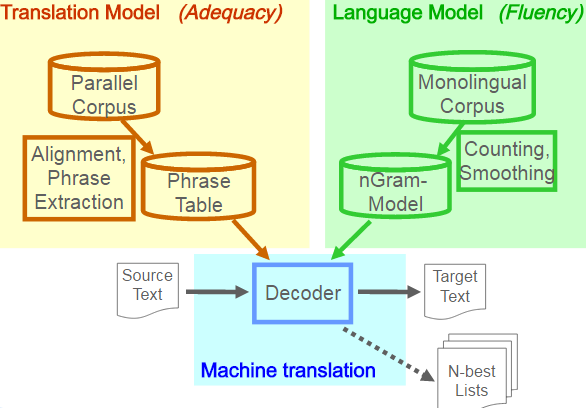
\includegraphics[width=0.6\linewidth]{figure/statml_architecture.PNG}
\label{fig:statml_architecture}
%\caption{}
\end{figure}
\end{frame}

%------------------------------------------------

\begin{frame} \frametitle{Open Source Language Models Example}
Architecture of the LIMSI SMT
system\footnote{http://www.limsi.fr/tlp/mt/} and open language models:
\begin{itemize}
\item SRILM\footnote{http://sourceforge.net/projects/irstlm/} (N-Gram)
  \& NN[Neural Networks] (Continuous Space LM).
\item Giza++: Translation Model. 
\item Moses: Decoder
\end{itemize}
\begin{figure}
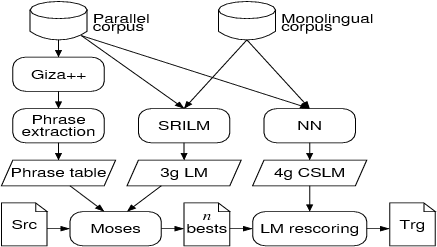
\includegraphics[width=0.6\linewidth]{figure/TLP_SMT_arch.png}
\label{fig:TLP_SMT_arch}
%\caption{}
\end{figure}
\end{frame}

%------------------------------------------------
\begin{frame}\frametitle{Other Language Models Applications}

\begin{block}{Speech Recognition}
  \quad $P_{LM}(\text{I saw a van}) > P_{LM}(\text{eyes awe of an})$
\end{block}

\begin{block}{Spell Correction}
The office is about fifteen minuets from my house. \\
  \quad $P_{LM}(\text{about fifteen minutes from}) >
  P_{LM}(\text{about fifteen minuets from})$
\end{block}

\begin{block}{Information Retrieval}
No results found for ``University of Brandeis'' (Query likelihood model).
  \quad $P_{LM}(\text{University of Brandeis}) >
  P_{LM}(\text{Brandeis University})$
\end{block}

\begin{block}{More !!}
Part-of-speech Tagging, Parsing, Summarization, Question-Answering,
etc.
\end{block}
\end{frame}

%------------------------------------------------
%%%%%%%%%%%%%%%%%%%%%%%%%%%%%%%%%%%%%%%%%%%%%%%%%%%%%%%%%%%%%%%%%%%%%

\section{N-Gram Language Models}

%------------------------------------------------
\begin{frame}\frametitle{Probabilistic Language Modeling}

\begin{block}{How to Compute $P(W)$}
  \quad $P(W) = P(w_1,\ldots,w_m)$
\end{block}

\begin{block}{Probability of an upcoming word}
 \quad  $P(w_k|w_1, w_2, \ldots, w_{k-1})$
\end{block}

\begin{block}{Decomposing using Chain Rule}
  \quad $P(w_1,\ldots,w_m) = P(w_1)P(w_2|w_1)P(w_2|w_1, w_2)\ldots P(w_m|w_1, w_2, \ldots, w_{m-1})$
\end{block}

\begin{block}{Example}
\quad $P(\text{its water is so transparent}) = $ \\ $P(\text{its})
\times P(\text{water}|\text{its}) \times P(\text{is}|\text{its water})
\times P(\text{so}|\text{its water is}) \times $ \\
$P(\text{transparent}|\text{its water is so})$
\end{block}
\end{frame}

%------------------------------------------------


\begin{frame}\frametitle{Chain Rule Estimation}

\begin{block}{Joint Probability}
  \quad $P(w_1w_2\ldots w_m) = \prod P(w_i|w_1w_2\ldots w_i-1)$
\end{block}

\begin{block}{How to estimate?}
Maximum likelihood estimation: \\
 \quad  $P(\text{transparent}|\text{its water is so}) = $\\ 
$$\frac{Count(\text{its water is so transparent})}{Count(\text{its water is so})}$$
\end{block}

\begin{block}{Problems?}
\begin{itemize}
\item Sparse data: NO enough data for estimating.
\item Large space: HUGE possible sentences.
\end{itemize}
\end{block}

\end{frame}


%------------------------------------------------
\begin{frame}\frametitle{Markov Chain}

\begin{block}{Markov Assumption}
  Only previous history matters: \\
 \quad  $P(\text{transparent}|\text{its water is so}) =
 (\text{transparent}|\text{so})$  or maybe \\
 \quad  $P(\text{transparent}|\text{its water is so}) = 
 (\text{transparent}|\text{so})$  
\end{block}

\begin{block}{$k_{\text{th}}$ Order Markov Model}
 \quad $P(w_1w_2\ldots w_m) = \prod P(w_i|w_{i-k}w_2\ldots w_i-1)$
\end{block}

\begin{block}{Simple Cases}
Unigram model:
 \quad $P(w_1w_2\ldots w_m) = \prod P(w_i)$

Bigram model:
 \quad $P(w_1w_2\ldots w_m) = \prod P(w_i|w_{i-1})$
\end{block}

\end{frame}


%------------------------------------------------

%------------------------------------------------
\begin{frame}\frametitle{N-gram Models}

\begin{block}{Is Markov assumption sufficient? \alert{NO!}}
Language has long-distance dependencies:

\begin{figure}
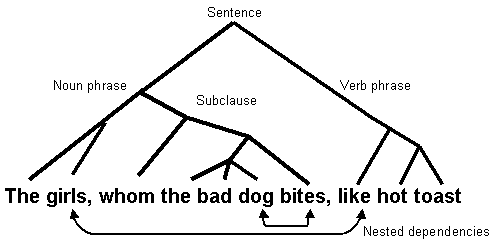
\includegraphics[width=0.6\linewidth]{figure/long-distance-dependency.png}
\label{fig:long-distance-dependency}
\end{figure}

Or:  \\

``The computer which I had just put into the machine room on the fifth
floor crashed.'' 

\end{block}
\end{frame}


%------------------------------------------------
%------------------------------------------------
\begin{frame}\frametitle{Bigram Example}
\begin{figure}
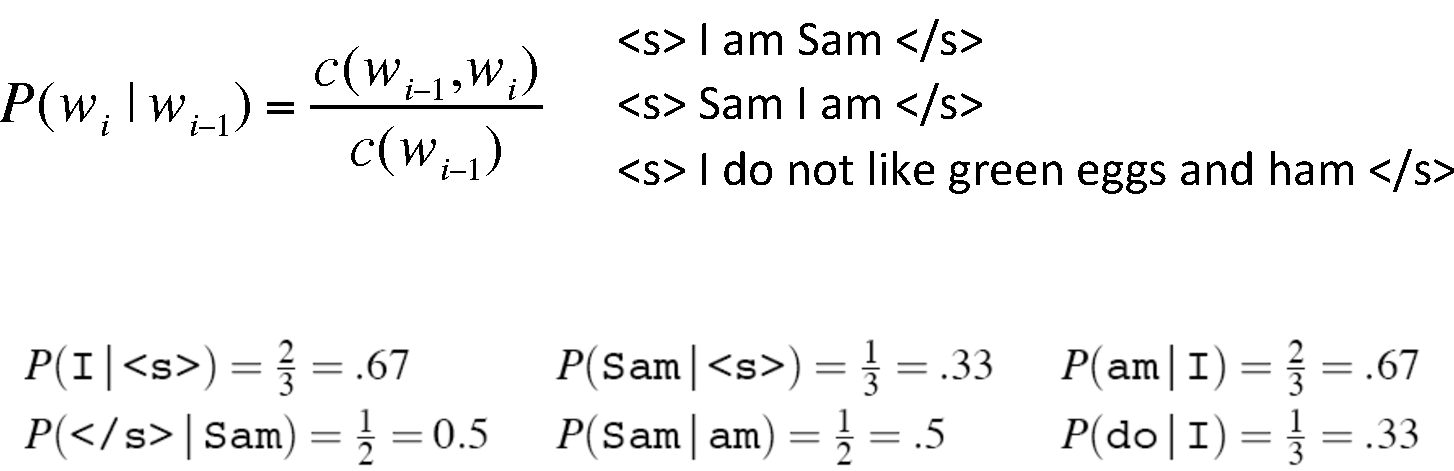
\includegraphics[width=1\linewidth]{figure/bigram_example.pdf}
\label{fig:bigram_example}
\end{figure}

\end{frame}


%------------------------------------------------
%------------------------------------------------
\begin{frame}\frametitle{Trigram Example}
\begin{figure}
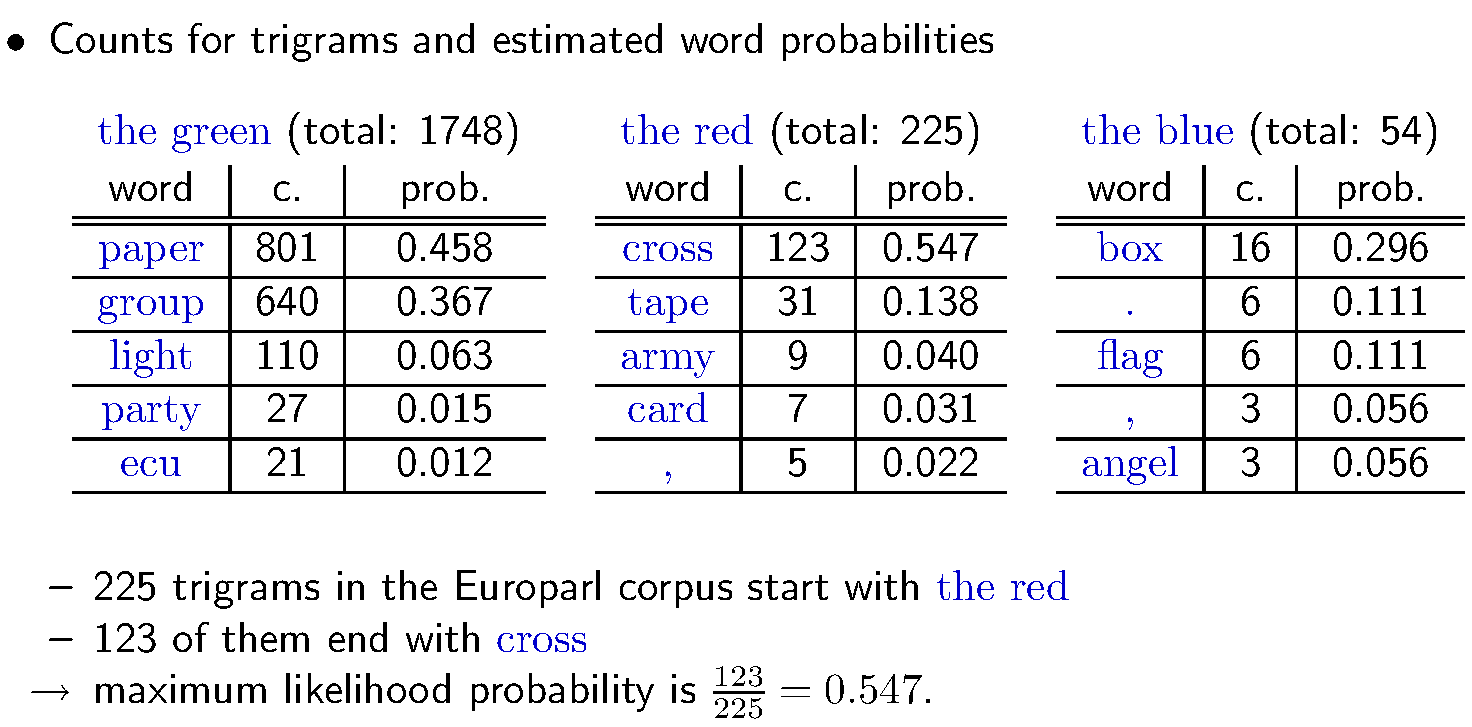
\includegraphics[width=1\linewidth]{figure/trigram_example.pdf}
\label{fig:trigram_example}
\end{figure}

``The red cross'' and ``The green party'' are frequent trigrams in the
Europarl corpus.
\end{frame}


%------------------------------------------------

%------------------------------------------------
\begin{frame}\frametitle{Evaluation of N-gram Models}

\begin{block}{How good is our model?}
Extrinsic Evaluation: training A \& B, testing, comparing accuracy of
A \& B by evaluation metric. \\

But it is \alert{time-consuming}.
\end{block}

\begin{block}{Intrinsic Evaluation}
Perplexity: How well can we predict the next word?

Intrinsic evaluation is \alert{Bad approximation}!
Unless the test data looks just like the training data. 

But is helpful to think about. 
\end{block}

\begin{block}{Intuition of Perplexity}
How hard is the task of recognizing digits ``0, 1, 2, 3, 4, 5, 6, 7,
8, 9''?

Perplexity 10.


\end{block}
\end{frame}


%------------------------------------------------
%------------------------------------------------
\begin{frame}\frametitle{Perplexity}

\begin{block}{Cross Entropy}
\begin{align*}
& H(W) =  -\frac{1}{n}\log{P(w_1w_2\ldots w_n)}  \\
& = -\frac{1}{n}\sum_i^n\log{P(w_i|w_1\ldots,w_{i-1})} 
\end{align*}
Perplexity:
$$
PP(W) = 2^{H(W)} = P(W)^{-\frac{1}{n}}
$$
\end{block}

\begin{block}{Perplexity as branching factor}
\begin{align*}
& PP(W) =  P(1\text{, }2\text{, }\ldots\text{, } 10)^{-\frac{1}{10}}  \\
& =(\frac{1}{10})^{10\times -\frac{1}{10}} = (\frac{1}{10})^{-1} = 10 
\end{align*}
\end{block}

\end{frame}


%------------------------------------------------
%------------------------------------------------
\begin{frame}\frametitle{Comparison N-gram Models}

Minimizing perplexity is the same as maximizing probability, thus
better model.

\begin{figure}
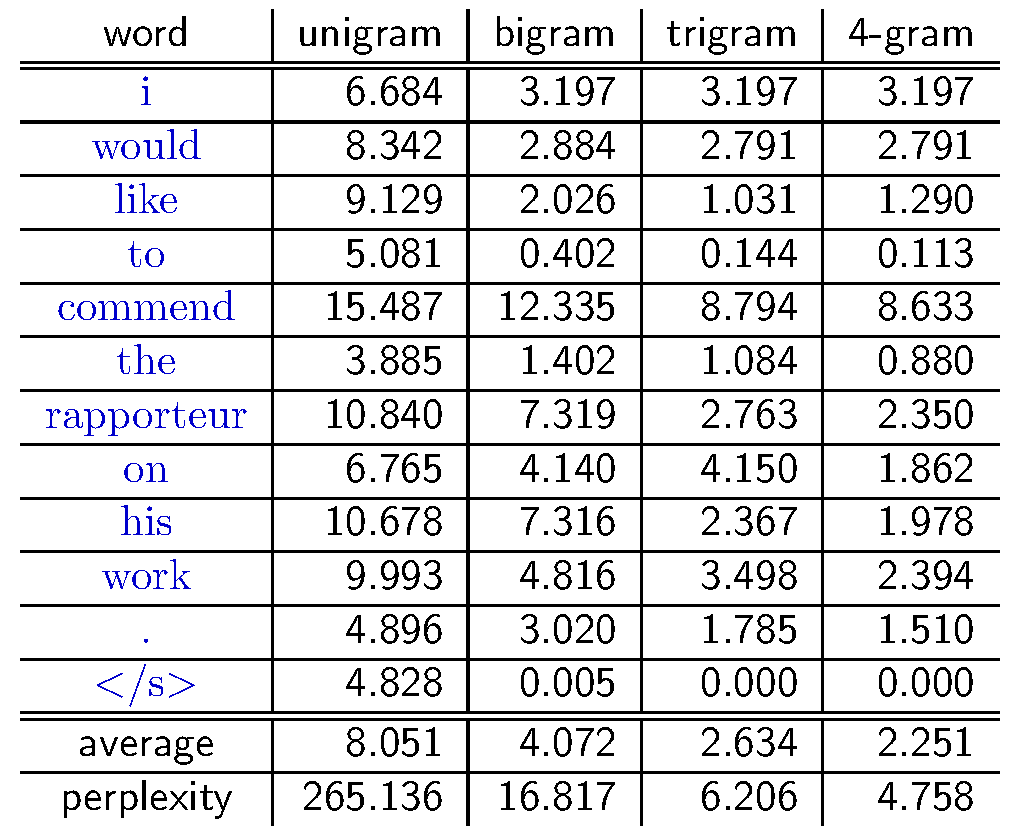
\includegraphics[width=0.6\linewidth]{figure/comparison_perplexity.pdf}
\label{fig:comparison_perplexity}
\end{figure}

\end{frame}


%------------------------------------------------
%------------------------------------------------
\begin{frame}\frametitle{Generalization and Zeros}

\begin{block}{Unseen N-grams}
Things that NOT ever occur in the training set. But occur in the test
set. 

\end{block}

\begin{columns}[t] % The "c" option specifies centered vertical alignment while the "t" option is used for top vertical alignment
\column{.45\textwidth} % Left column and width
Training Set:
\begin{enumerate}
\item ... denied the allegations
\item ... denied the reports
\item ... denied the claims
\item ... denied the request
\end{enumerate}

\column{.5\textwidth} % Right column and width
Test Set:
\begin{enumerate}
\item ... denied the offer
\item ... denied the loan
\end{enumerate}
\end{columns}
$$
P(\text{``offer''}|\text{''denied the''}) = 0
$$

\begin{block}{Smoothing}
Sparse statistics, smoothing to generalize better.
\end{block}
\end{frame}


%------------------------------------------------
%------------------------------------------------
\begin{frame}\frametitle{Smoothing}

\begin{block}{How to smooth all words non-zeros}

\begin{figure}
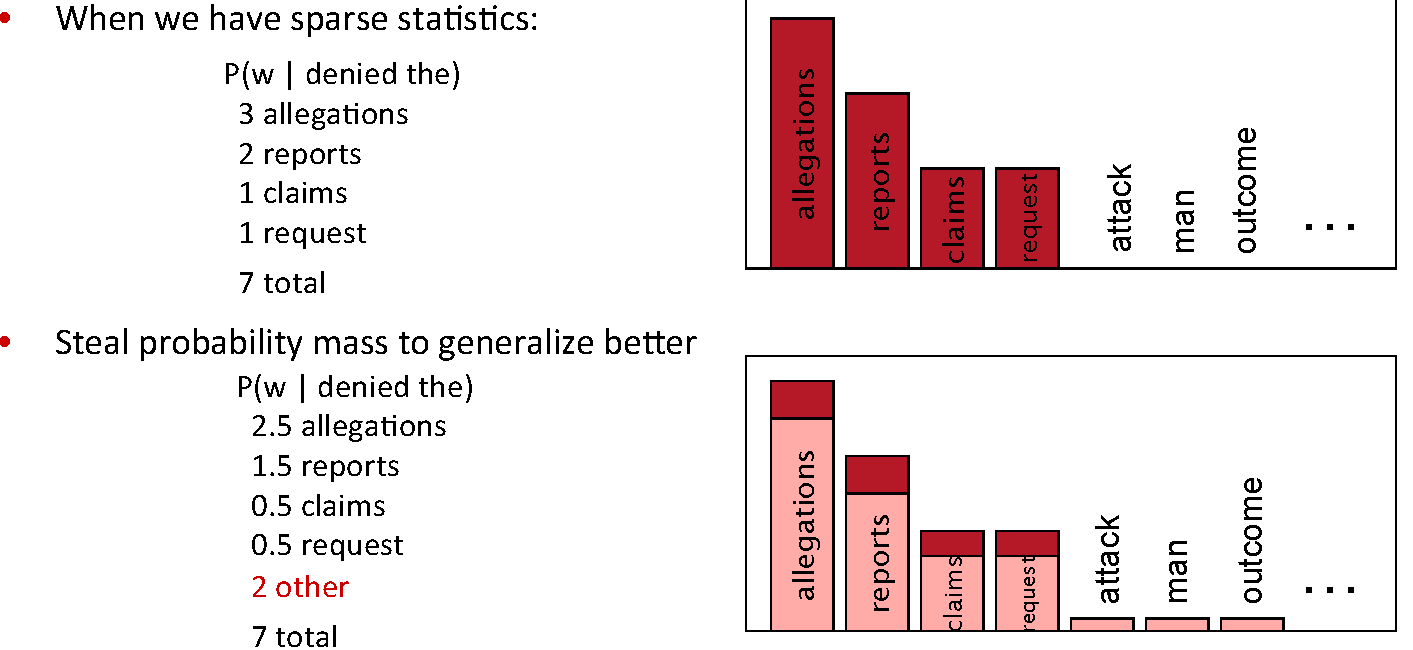
\includegraphics[width=0.9\linewidth]{figure/smoothing.pdf}
\label{fig:smoothing}
\end{figure}
\end{block}
\end{frame}


%------------------------------------------------
%------------------------------------------------
\begin{frame}\frametitle{Add-One Smoothing}

\begin{block}{Laplace smoothing}
Pretend we saw each word one more time than we did.

\begin{figure}
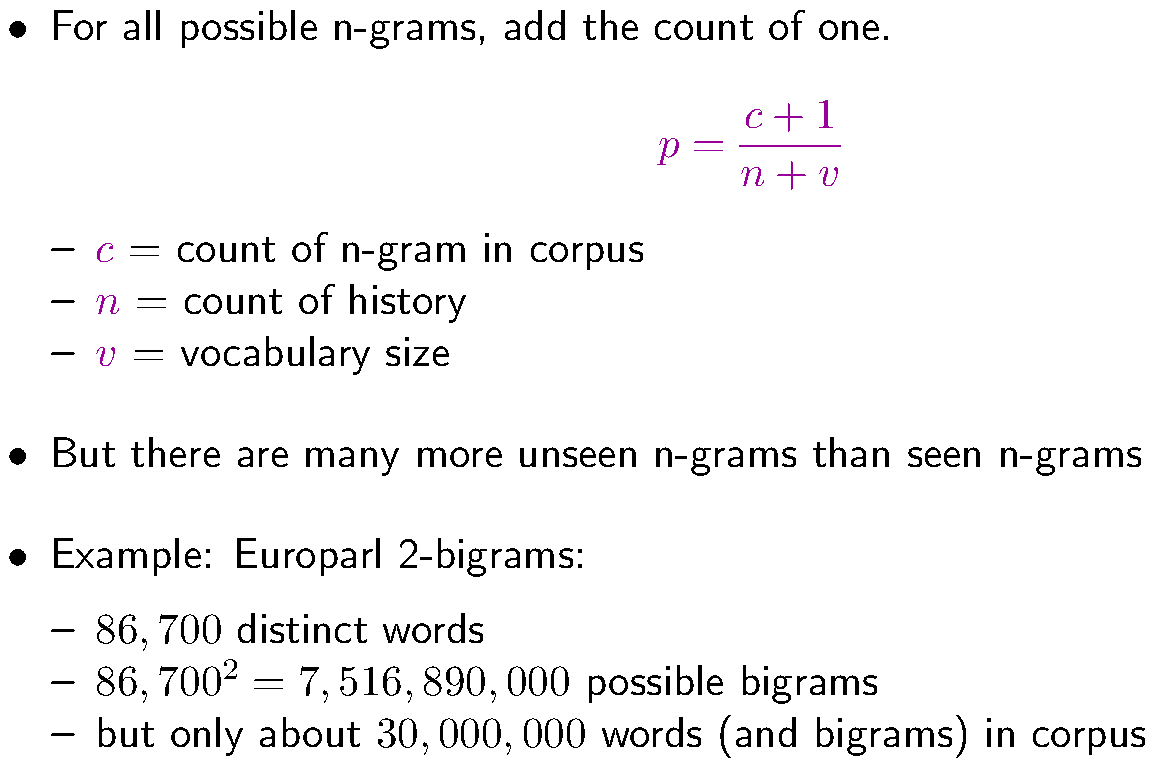
\includegraphics[width=0.6\linewidth]{figure/laplace_smoothing.pdf}
\label{fig:laplace_smoothing}
\end{figure}

\end{block}
\end{frame}


%------------------------------------------------
%------------------------------------------------
\begin{frame}\frametitle{Bigram Add-One Smoothing}
\begin{figure}
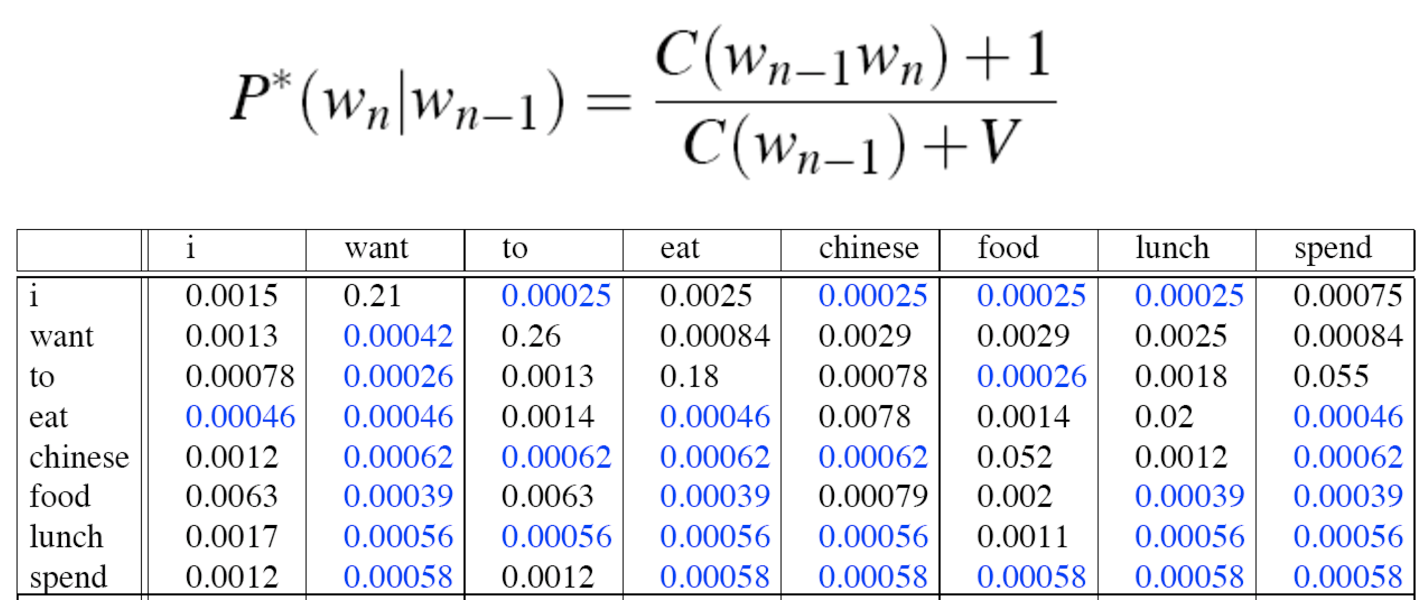
\includegraphics[width=0.9\linewidth]{figure/bigram_addone_smoothing.pdf}
\label{fig:bigram_addone_smoothing}
\end{figure}

\end{frame}


%------------------------------------------------
%------------------------------------------------
\begin{frame}\frametitle{Add-$\alpha$ Smoothing}

\begin{block}{Will $\alpha$ adjusted count a lot?}
\begin{figure}
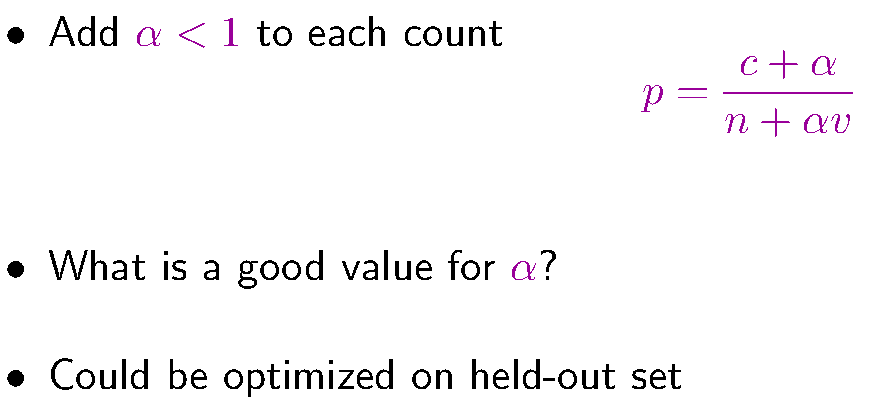
\includegraphics[width=0.8\linewidth]{figure/add_alpha_smoothing.pdf}
\label{fig:add_alpha_smoothing}
\end{figure}
\end{block}

\end{frame}


%------------------------------------------------
%------------------------------------------------
\begin{frame}\frametitle{Comparison of Add-$\alpha$ Smoothing}

\begin{block}{Bigram in Europarl corpus}

\begin{figure}
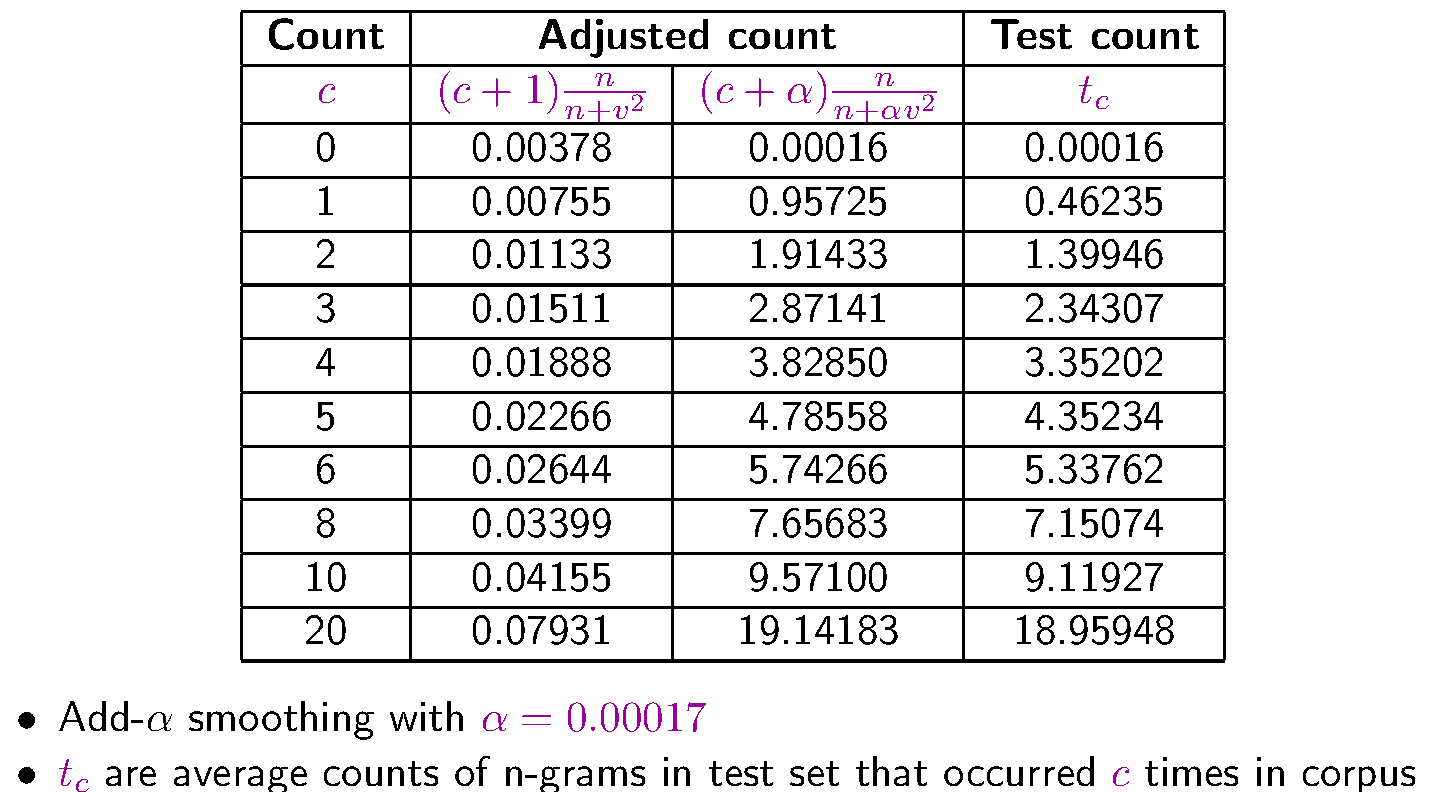
\includegraphics[width=0.9\linewidth]{figure/bigram_alpha_smoothing.pdf}
\label{fig:bigram_alpha_smoothing}
\end{figure}

\end{block}
\end{frame}


%------------------------------------------------
%------------------------------------------------
\begin{frame}\frametitle{N-gram Models}

\begin{block}{Is Markov assumption sufficient? \alert{NO!}}
Language has long-distance dependencies:

\begin{figure}
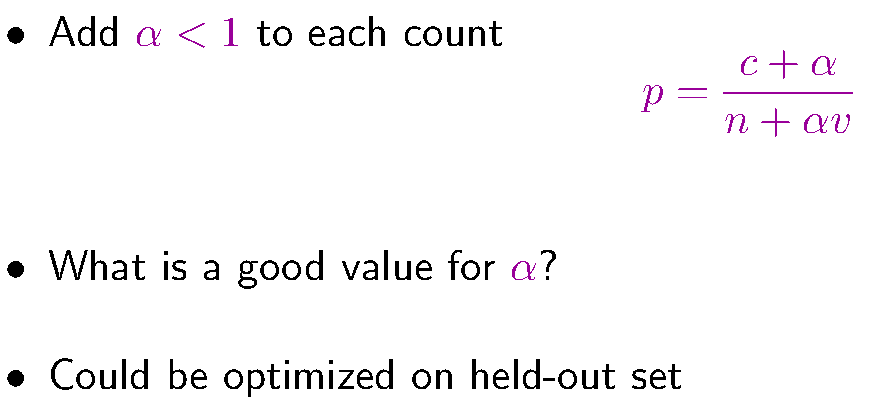
\includegraphics[width=0.6\linewidth]{figure/add_alpha_smoothing.pdf}
\label{fig:add_alpha_smoothing}
\end{figure}
\end{block}

\end{frame}


%------------------------------------------------
%------------------------------------------------
\begin{frame}\frametitle{Comparison of Add-$\alpha$ Smoothing}

\begin{block}{Bigram in Europarl corpus}

\begin{figure}
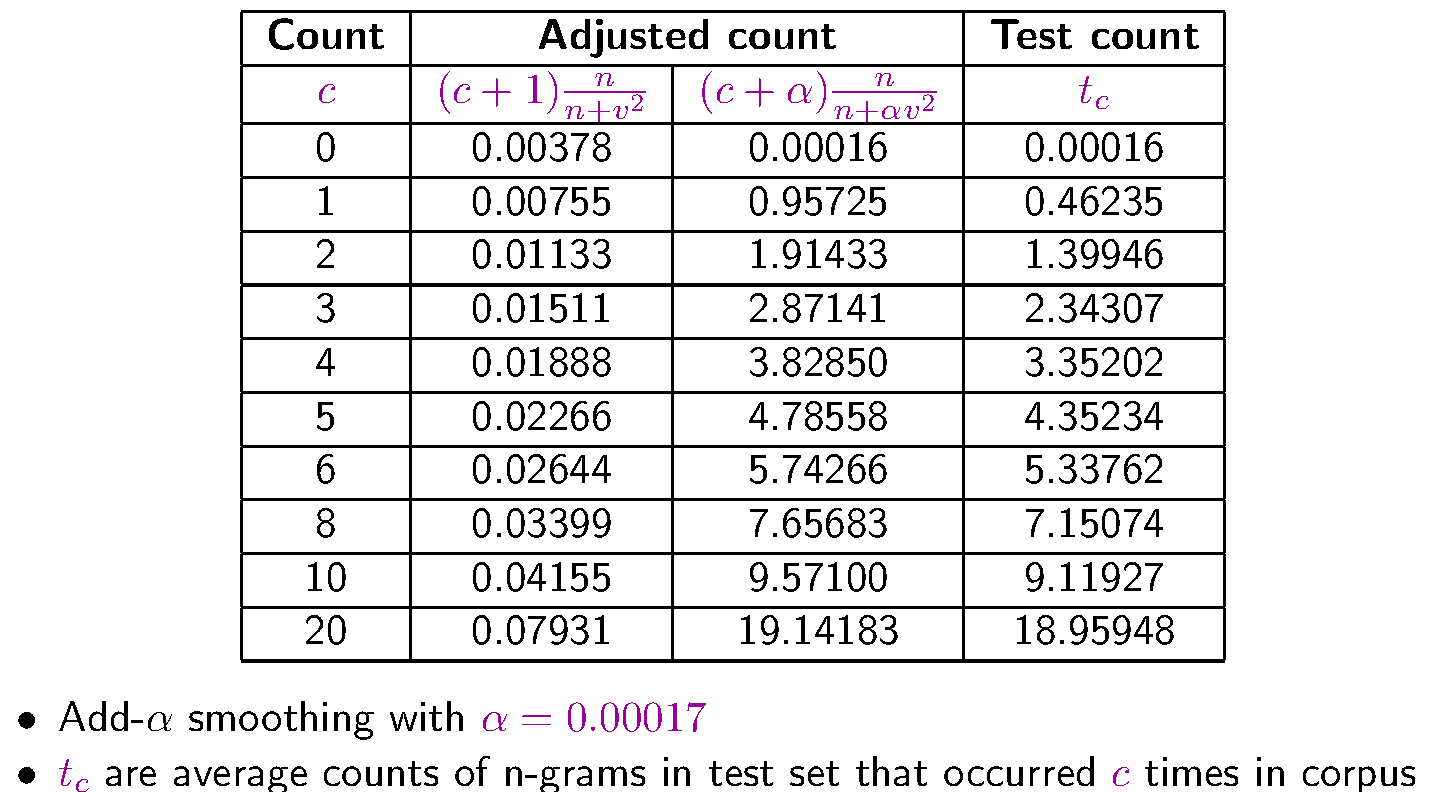
\includegraphics[width=0.9\linewidth]{figure/bigram_alpha_smoothing.pdf}
\label{fig:bigram_alpha_smoothing}
\end{figure}

\end{block}
\end{frame}


%------------------------------------------------
%------------------------------------------------
\begin{frame}\frametitle{Held-out Estimation}

\begin{block}{Long Tail of N-gram Counting}
\begin{itemize}
\item 1,266,566 bigrams in this corpus, more than
half, 753,777, occur only once.
\item Zipf's Law:  the frequency of any word is inversely proportional to its rank in the frequency table. 
\end{itemize}

If we observe an n-gram
c times in the training corpus, ow often
do we expect it to see in the future (Held-out Estimation)?

$p_h(w_1w_2\ldots w_n) = \frac{E[r]}{N_h} \sim \frac{T_r}{N_r\times
  N_h}$,
$r = count_h(w_1w_2\ldots w_n)$
\end{block}

\begin{block}{Cross-Validation Estimation}
$$E(r) = \frac{T_r^1+T_r^2}{N_r^1+N_r^2}$$
\end{block}


\end{frame}


%------------------------------------------------
%------------------------------------------------
\begin{frame}\frametitle{Deleted Estimation}

Deleted Estimation: leave one part of the training corpus out
for validation.

\begin{columns}[c] % The "c" option specifies centered vertical alignment while the "t" option is used for top vertical alignment
\column{.5\textwidth} % Left column and width

\begin{figure}
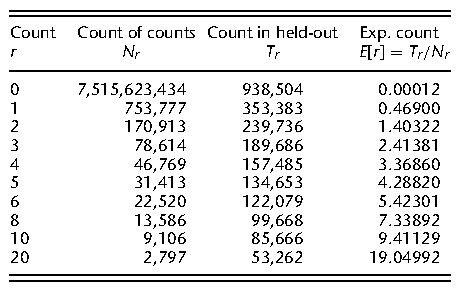
\includegraphics[width=0.9\linewidth]{figure/deleted_estimation.pdf}
\label{fig:deleted_estimation}
\end{figure}

\column{.5\textwidth} % Right column and width

\begin{figure}
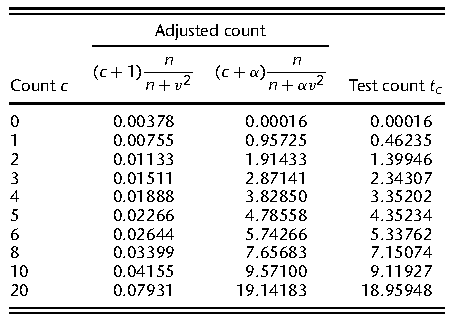
\includegraphics[width=0.9\linewidth]{figure/test_count.pdf}
\label{fig:test_acount}
\end{figure}

\end{columns}

\end{frame}


%------------------------------------------------
%%%%%%%%%%%%%%%%%%%%%%%%%%%%%%%%%%%%%%%%%%%%%%%%%%%%%%%%%%%%%%%%%%%%%
\section{Smoothing}


%------------------------------------------------
\begin{frame}\frametitle{Good-Turing Smoothing Intuition}
\begin{figure}
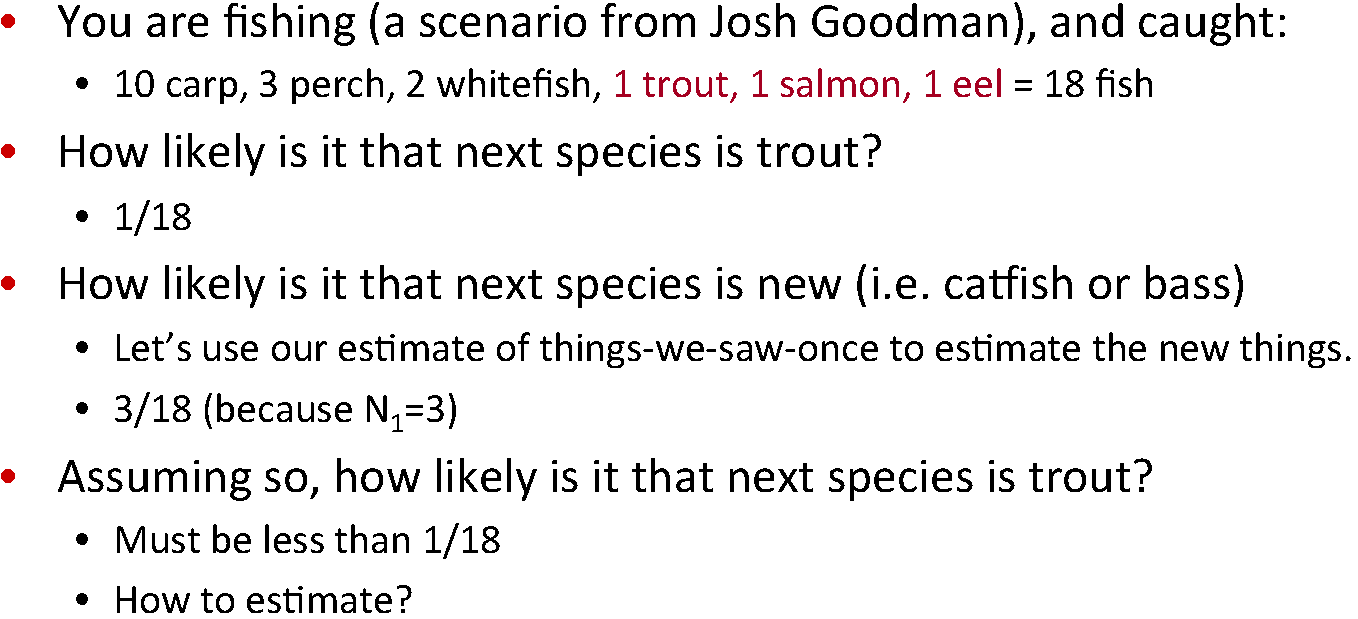
\includegraphics[width=1\linewidth]{figure/good_turing_smoothing.pdf}
\label{fig:good_turing_smoothing}
\end{figure}
\end{frame}


%------------------------------------------------
%------------------------------------------------
\begin{frame}\frametitle{Good-Turing Smoothing Calculation}
\begin{figure}
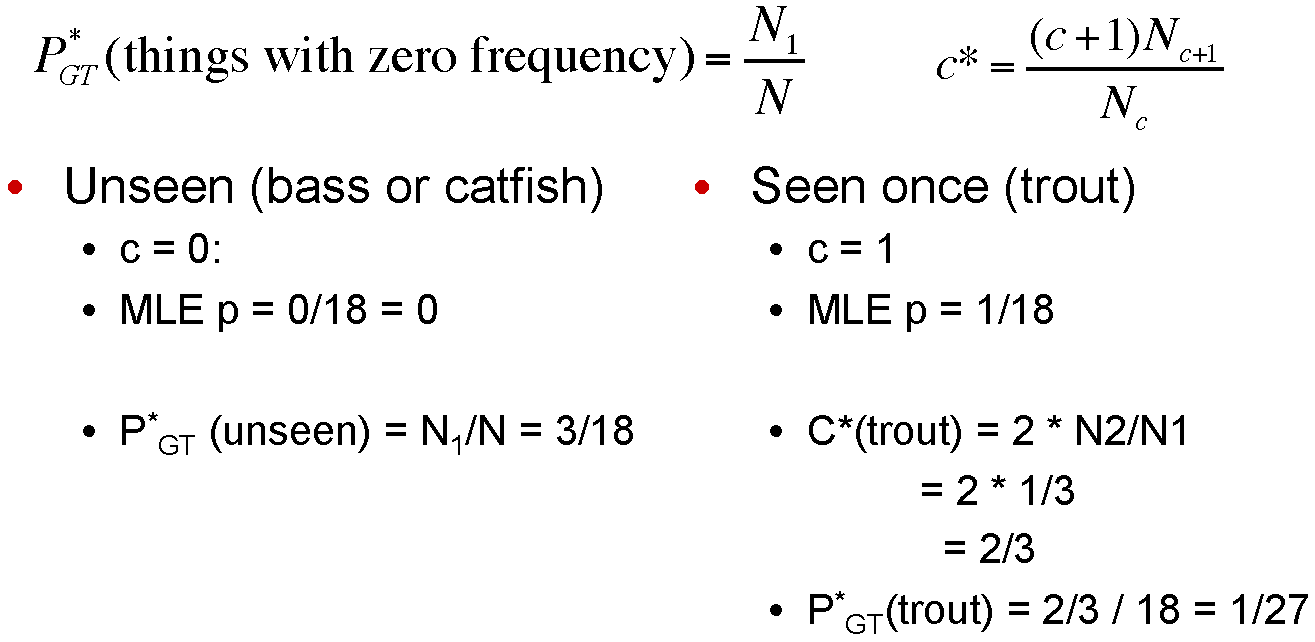
\includegraphics[width=0.9\linewidth]{figure/good_turing_calculation.pdf}
\label{fig:good_turing_calculation}
\end{figure}
\end{frame}


%------------------------------------------------
%------------------------------------------------
\begin{frame}\frametitle{Leave One Out Intuition}
\begin{figure}
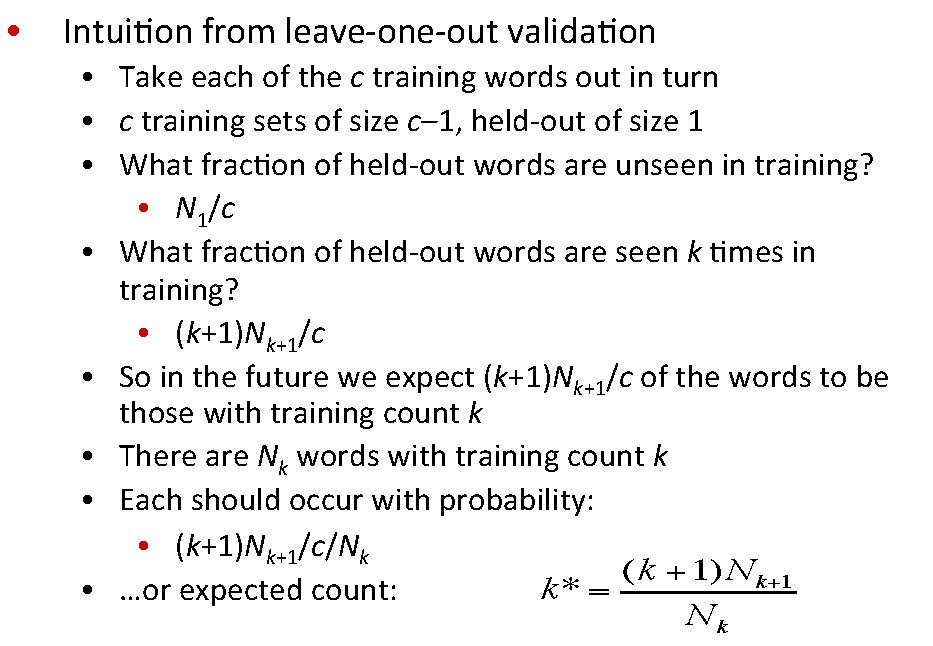
\includegraphics[width=0.9\linewidth]{figure/good_turing_loo_intuition.pdf}
\label{fig:good_turing_loo_intuition}
\end{figure}
\end{frame}


%------------------------------------------------
%------------------------------------------------
\begin{frame}\frametitle{Good-Turing for 2-Grams in Europarl}
\begin{figure}
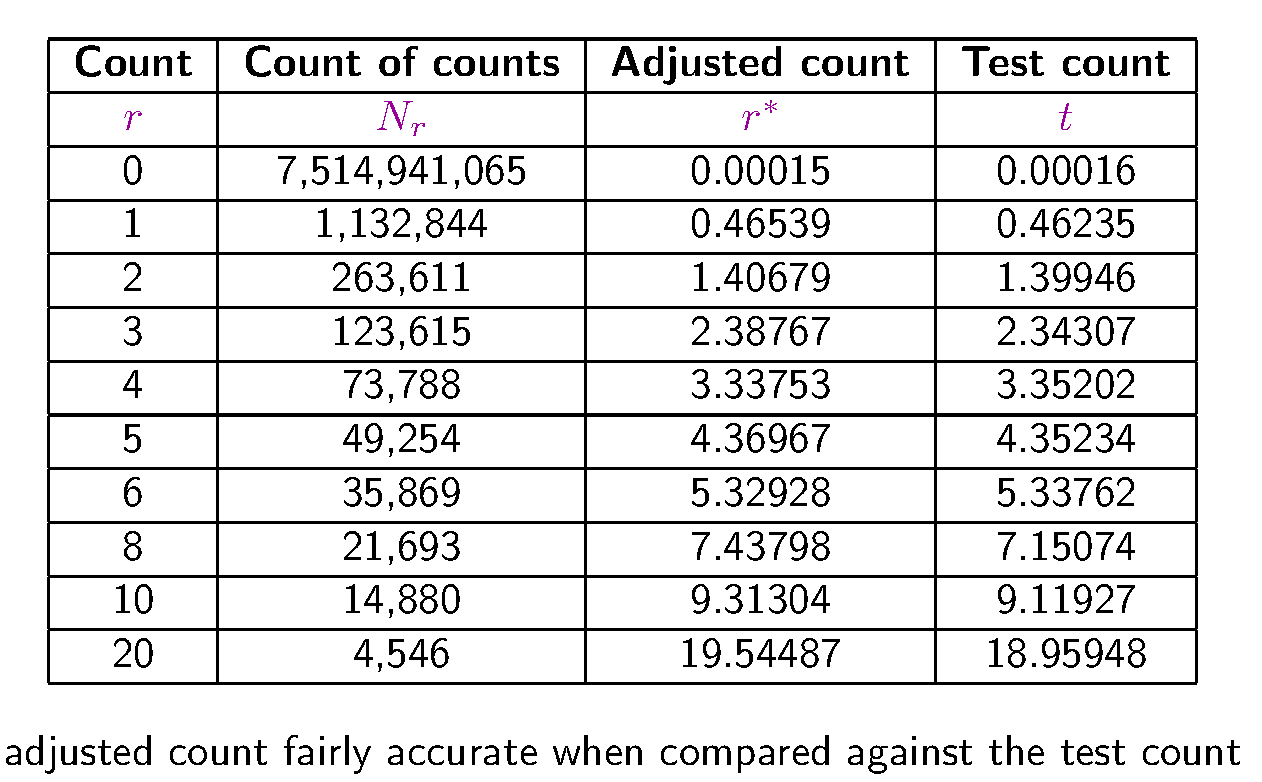
\includegraphics[width=0.9\linewidth]{figure/good_turing_2gram.pdf}
\end{figure}
\end{frame}


%------------------------------------------------
%------------------------------------------------
\begin{frame}\frametitle{Derivation of Good-Turing}
\begin{figure}
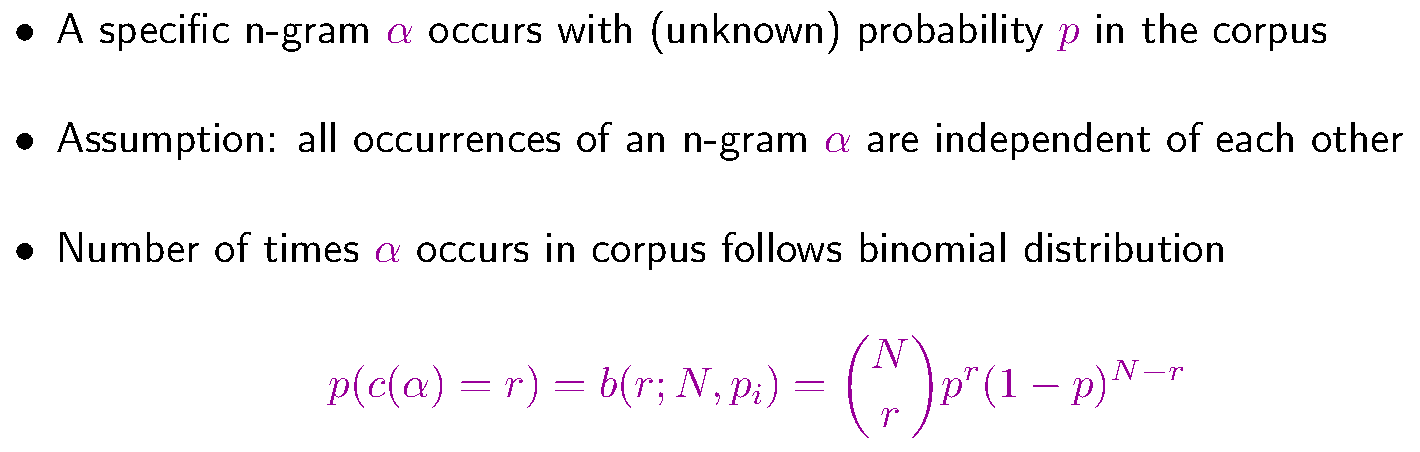
\includegraphics[width=0.9\linewidth]{figure/derivation_good_turing.pdf}
\end{figure}
\end{frame}


%------------------------------------------------
%------------------------------------------------
\begin{frame}\frametitle{Derivation of Good-Turing (2)}
\begin{figure}
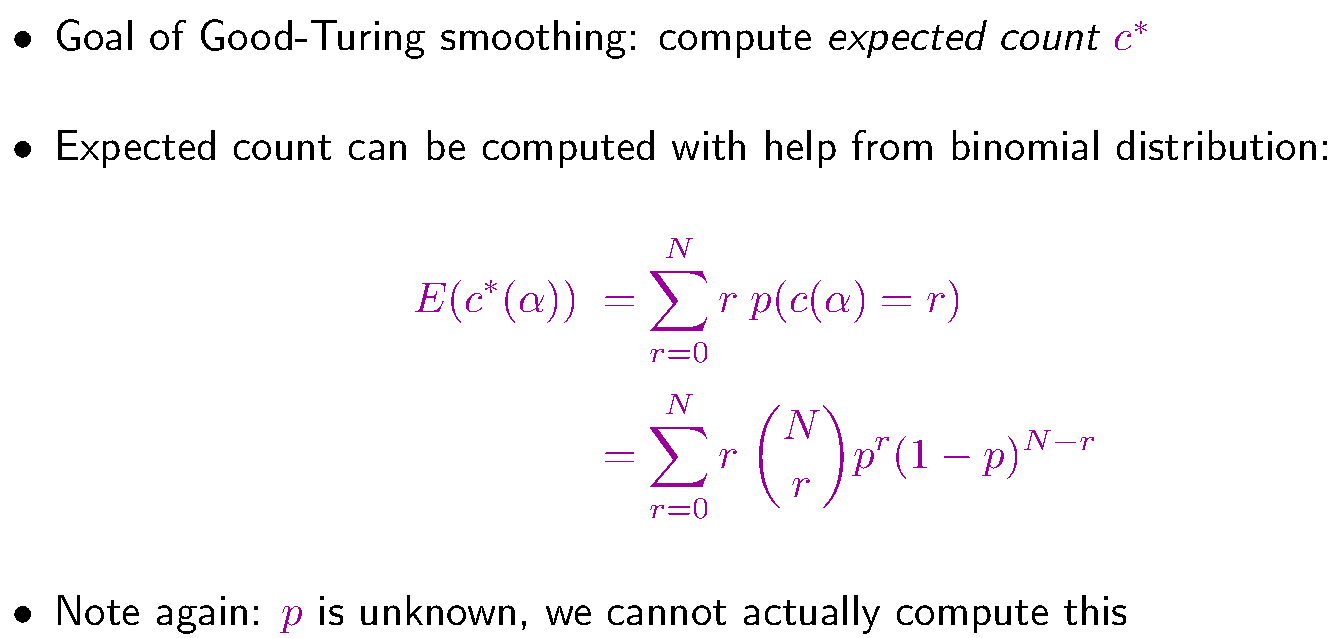
\includegraphics[width=0.9\linewidth]{figure/derivation_good_turing_2.pdf}
\end{figure}
\end{frame}


%------------------------------------------------
%------------------------------------------------
\begin{frame}\frametitle{Derivation of Good-Turing (3)}
\begin{figure}
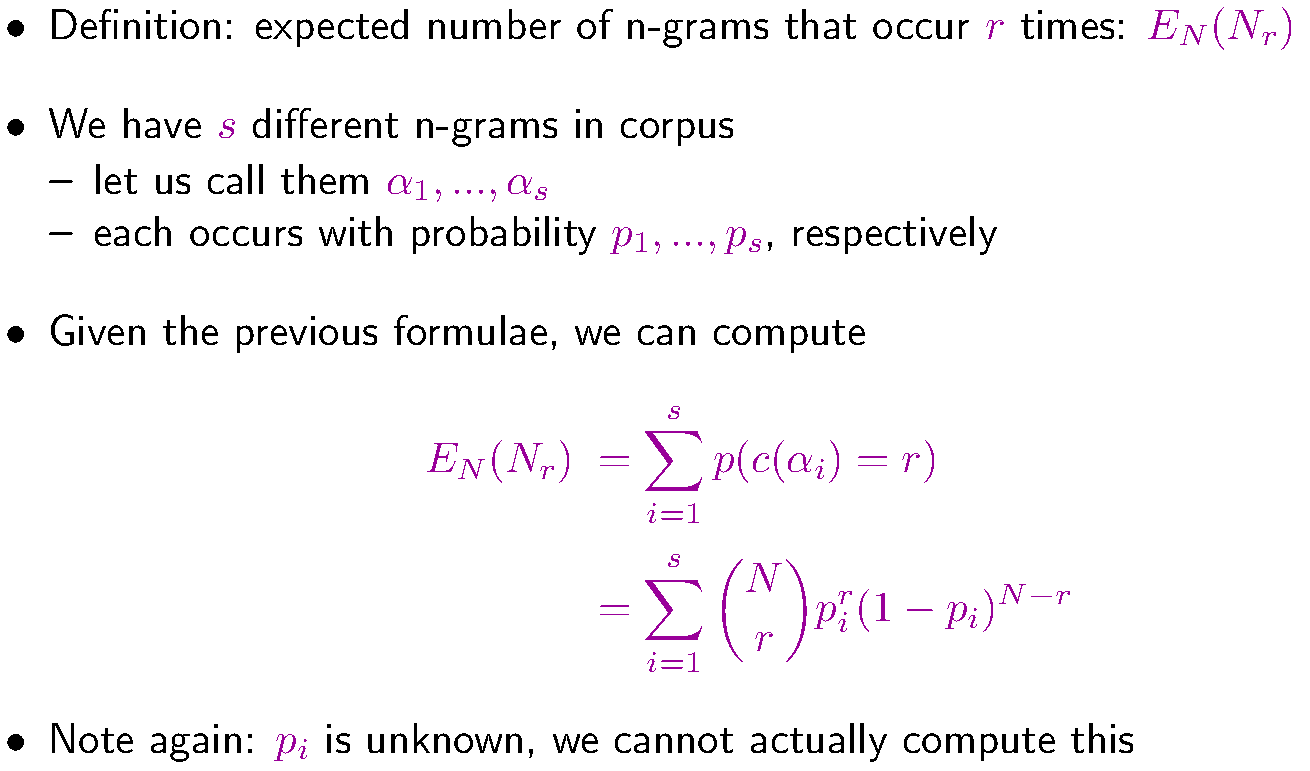
\includegraphics[width=0.9\linewidth]{figure/derivation_good_turing_3.pdf}
\end{figure}
\end{frame}


%------------------------------------------------
%------------------------------------------------
\begin{frame}\frametitle{Derivation of Good-Turing (4)}
\begin{figure}
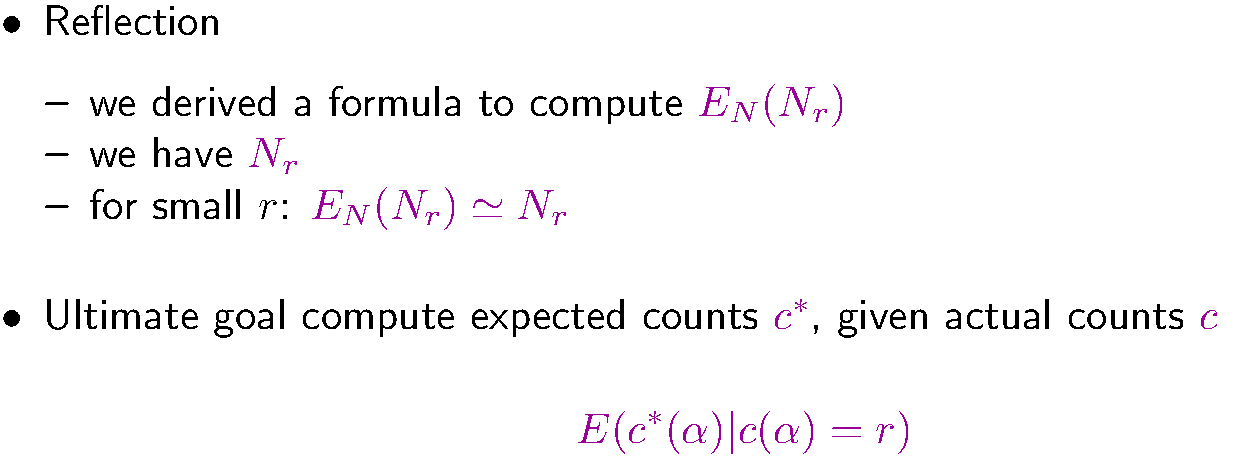
\includegraphics[width=0.9\linewidth]{figure/derivation_good_turing_4.pdf}
\end{figure}
\end{frame}


%------------------------------------------------
%------------------------------------------------
\begin{frame}\frametitle{Derivation of Good-Turing (5)}
\begin{figure}
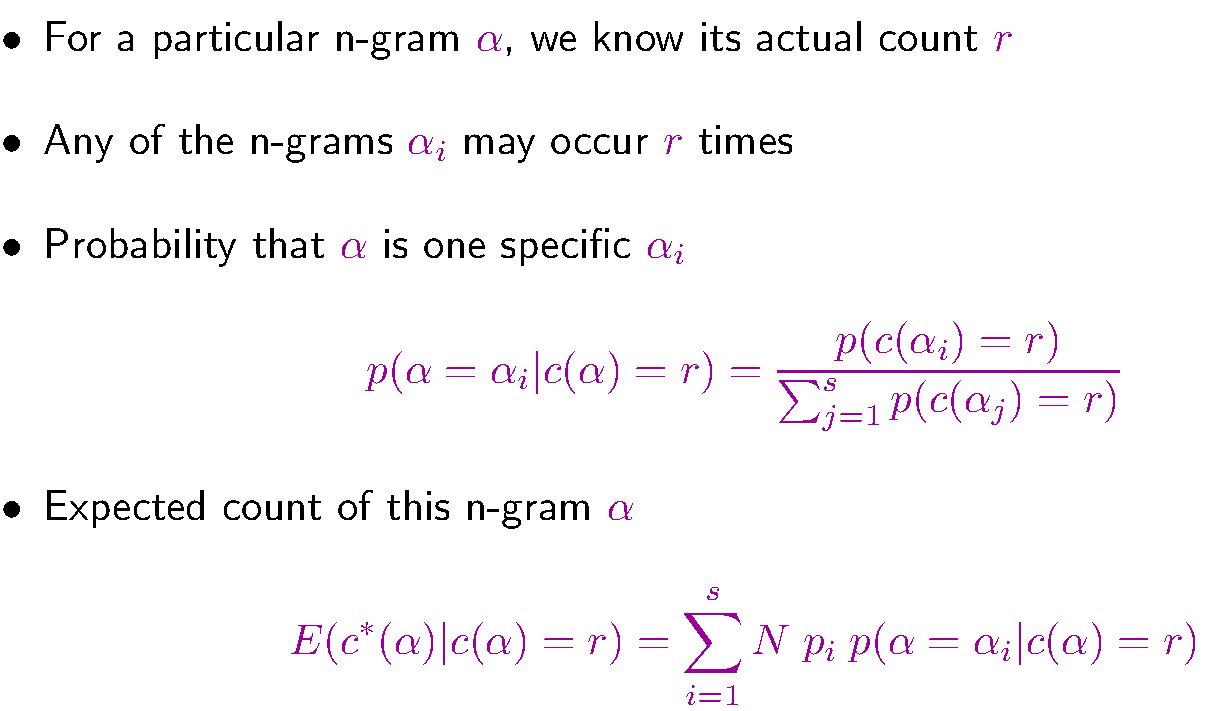
\includegraphics[width=0.9\linewidth]{figure/derivation_good_turing_5.pdf}
\end{figure}
\end{frame}


%------------------------------------------------
%------------------------------------------------
\begin{frame}\frametitle{Derivation of Good-Turing (6)}
\begin{figure}
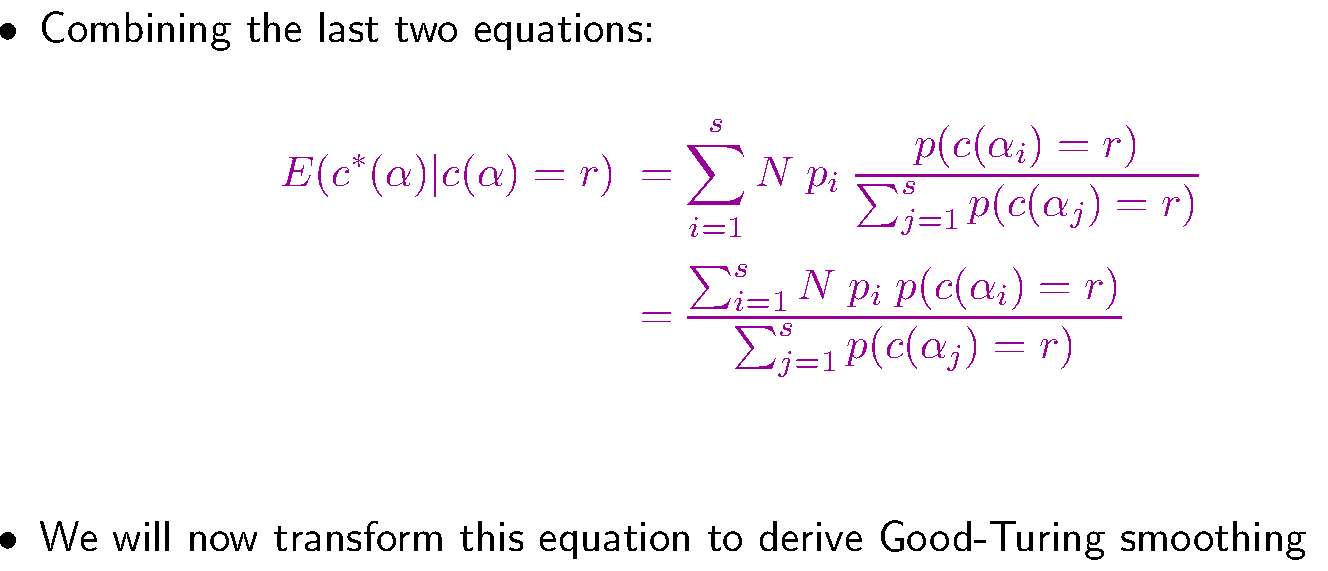
\includegraphics[width=0.9\linewidth]{figure/derivation_good_turing_6.pdf}
\end{figure}
\end{frame}


%------------------------------------------------
%------------------------------------------------
\begin{frame}\frametitle{Derivation of Good-Turing (7)}
\begin{figure}
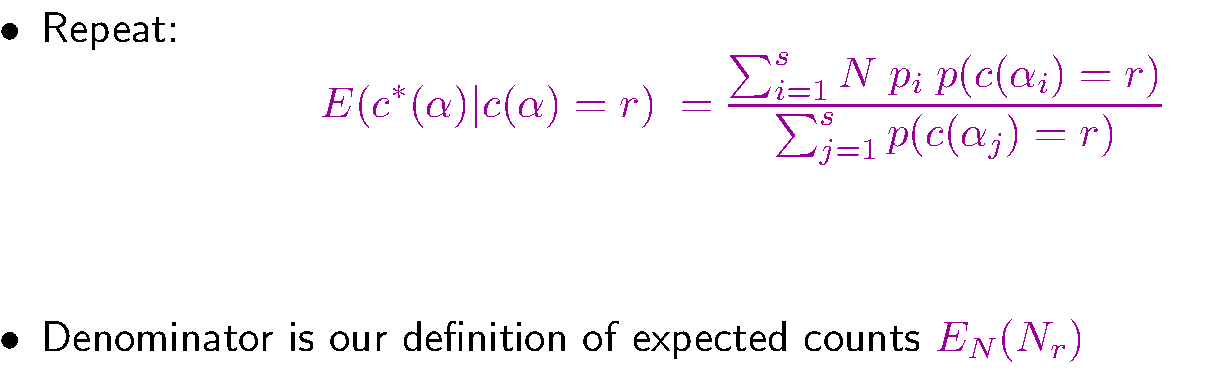
\includegraphics[width=0.9\linewidth]{figure/derivation_good_turing_7.pdf}
\end{figure}
\end{frame}


%------------------------------------------------
%------------------------------------------------
\begin{frame}\frametitle{Derivation of Good-Turing (8)}
\begin{figure}
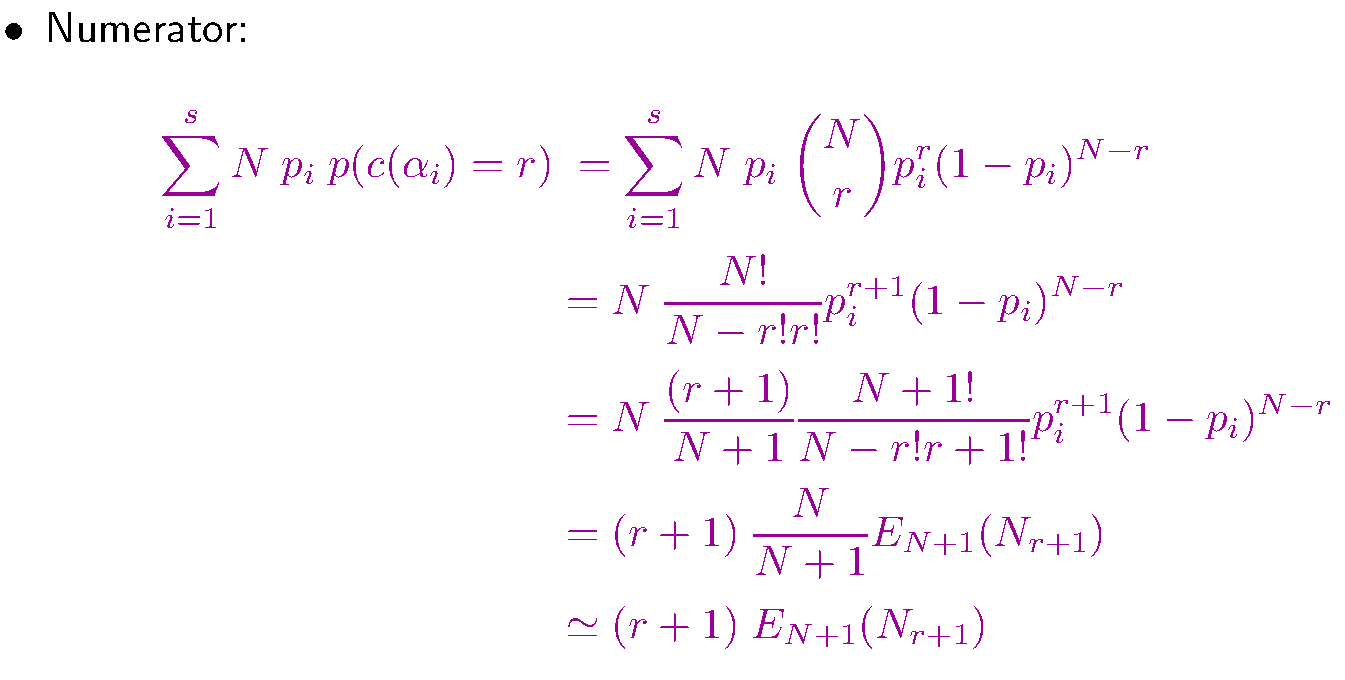
\includegraphics[width=0.9\linewidth]{figure/derivation_good_turing_8.pdf}
\end{figure}
\end{frame}


%------------------------------------------------
%------------------------------------------------
\begin{frame}\frametitle{Derivation of Good-Turing (9)}
\begin{figure}
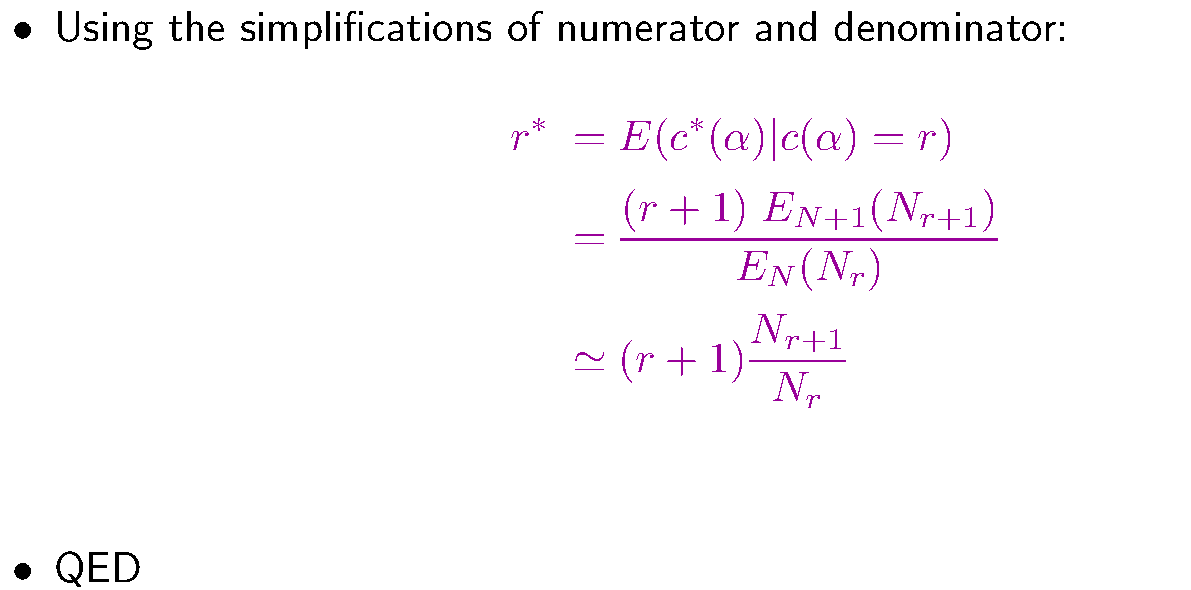
\includegraphics[width=0.9\linewidth]{figure/derivation_good_turing_9.pdf}
\end{figure}
\end{frame}


%------------------------------------------------



%%%%%%%%%%%%%%%%%%%%%%%%%%%%%%%%%%%%%%%%%%%%%%%%%%%%%%%%%%%%%%%%%%%%%
\section{Interpolation \& Back-off}



%------------------------------------------------
\begin{frame}\frametitle{Interpolation \& Back-off}

\begin{block}{Sparseness in a Trigram Model}

\begin{enumerate}
\item Back to bigrams, otherwise unigram: \alert{Back-off}
\item Mix that model with bigram and unigram: \alert{Interpolation} 
\end{enumerate}

\end{block}


\begin{block}{Context}
\begin{enumerate}
\item \alert{Back-off}: 
some times it helps to use less
context condition on less context for contexts
you haven't learned much about.

\item \alert{Interpolation}: 
higher and lower order n-gram models have different strengths and weaknesses:
\begin{itemize}
\item high-order n-grams are sensitive to more context, but have sparse counts.
\item low-order n-grams consider only very limited context, but have robust counts
\end{itemize}
\end{enumerate}

\end{block}


\end{frame}


%------------------------------------------------
%------------------------------------------------
\begin{frame}\frametitle{Interpola1on}

\begin{block}{Simple interpolation}
\vspace{-15pt}
\begin{align*}
\hat{P}(w_n|w_{n-1}w_{n-2})= & \lambda_1 P(w_n|w_{n-1}w_{n-2}) + \lambda_2 P(w_n|w_{n-1}) + \\
& (1-\lambda_1 - \lambda_2) P(w_n) 
\end{align*}
\end{block}

\begin{block}{Recursive Interpolation}
Lambdas conditional on context:
\vspace{-5pt}
\begin{align*}
\hat{P}(w_n|w_{n-1}w_{n-2})= & \lambda_1(w_{n-2}^{n-1}) P(w_n|w_{n-1}w_{n-2}) + \lambda_2(w_{n-2}^{n-1}) P(w_n|w_{n-1}) + \\
& (1-\lambda_1(w_{n-2}^{n-1}) - \lambda_2(w_{n-2}^{n-1})) P(w_n) 
\end{align*}
\vspace{-10pt}
{\footnotesize
\begin{align*}
\sum_{w\in V}\hat{P}(w_n|w_{n-1}w_{n-2})= &
\lambda_1(w_{n-2}^{n-1}) \sum_{w\in V}  P(w_n|w_{n-1}w_{n-2}) + \lambda_2(w_{n-2}^{n-1})\sum_{w\in V}  P(w_n|w_{n-1}) + \\
& (1-\lambda_1(w_{n-2}^{n-1}) -
\lambda_2(w_{n-2}^{n-1})) \sum_{w\in V} P(w_n)\\
& =  \lambda_1(w_{n-2}^{n-1}) + \lambda_2(w_{n-2}^{n-1}) + (1-\lambda_1(w_{n-2}^{n-1}) -
\lambda_2(w_{n-2}^{n-1})) = 1
\end{align*}
}%
\end{block}


\end{frame}


%------------------------------------------------
%------------------------------------------------
\begin{frame}\frametitle{N-gram Models}

\begin{block}{Is Markov assumption sufficient? \alert{NO!}}
Language has long-distance dependencies:

\begin{figure}
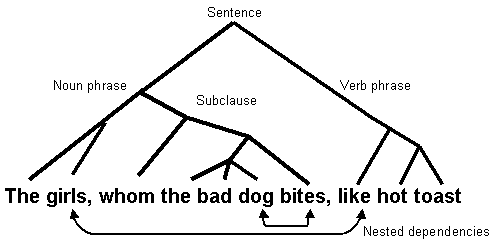
\includegraphics[width=0.6\linewidth]{figure/long-distance-dependency.png}
\label{fig:long-distance-dependency}
\end{figure}

Or:  \\

``The computer which I had just put into the machine room on the fifth
floor crashed.'' 

\end{block}
\end{frame}


%------------------------------------------------
%------------------------------------------------
\begin{frame}\frametitle{N-gram Models}

\begin{block}{Is Markov assumption sufficient? \alert{NO!}}
Language has long-distance dependencies:

\begin{figure}
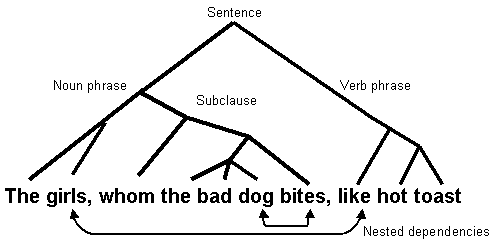
\includegraphics[width=0.6\linewidth]{figure/long-distance-dependency.png}
\label{fig:long-distance-dependency}
\end{figure}

Or:  \\

``The computer which I had just put into the machine room on the fifth
floor crashed.'' 

\end{block}
\end{frame}


%------------------------------------------------
%------------------------------------------------
\begin{frame}\frametitle{N-gram Models}

\begin{block}{Is Markov assumption sufficient? \alert{NO!}}
Language has long-distance dependencies:

\begin{figure}
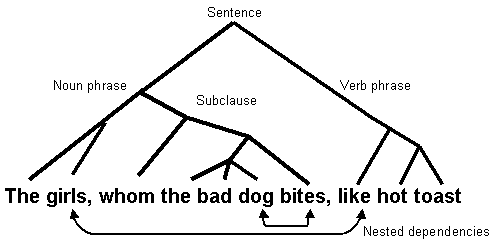
\includegraphics[width=0.6\linewidth]{figure/long-distance-dependency.png}
\label{fig:long-distance-dependency}
\end{figure}

Or:  \\

``The computer which I had just put into the machine room on the fifth
floor crashed.'' 

\end{block}
\end{frame}


%------------------------------------------------
%------------------------------------------------
\begin{frame}\frametitle{N-gram Models}

\begin{block}{Is Markov assumption sufficient? \alert{NO!}}
Language has long-distance dependencies:

\begin{figure}
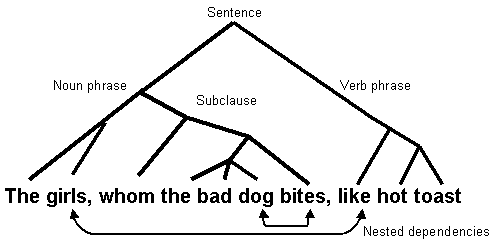
\includegraphics[width=0.6\linewidth]{figure/long-distance-dependency.png}
\label{fig:long-distance-dependency}
\end{figure}

Or:  \\

``The computer which I had just put into the machine room on the fifth
floor crashed.'' 

\end{block}
\end{frame}


%------------------------------------------------
%------------------------------------------------
\begin{frame}\frametitle{N-gram Models}

\begin{block}{Is Markov assumption sufficient? \alert{NO!}}
Language has long-distance dependencies:

\begin{figure}
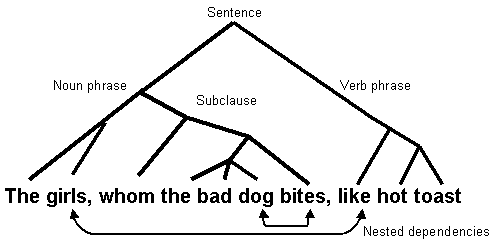
\includegraphics[width=0.6\linewidth]{figure/long-distance-dependency.png}
\label{fig:long-distance-dependency}
\end{figure}

Or:  \\

``The computer which I had just put into the machine room on the fifth
floor crashed.'' 

\end{block}
\end{frame}


%------------------------------------------------
%------------------------------------------------
\begin{frame}\frametitle{N-gram Models}

\begin{block}{Is Markov assumption sufficient? \alert{NO!}}
Language has long-distance dependencies:

\begin{figure}
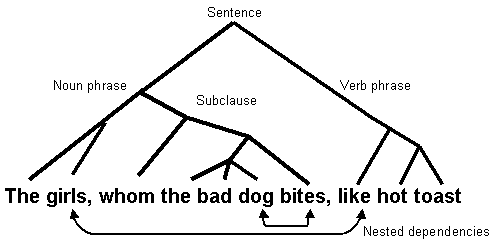
\includegraphics[width=0.6\linewidth]{figure/long-distance-dependency.png}
\label{fig:long-distance-dependency}
\end{figure}

Or:  \\

``The computer which I had just put into the machine room on the fifth
floor crashed.'' 

\end{block}
\end{frame}


%------------------------------------------------
%------------------------------------------------
\begin{frame}\frametitle{N-gram Models}

\begin{block}{Is Markov assumption sufficient? \alert{NO!}}
Language has long-distance dependencies:

\begin{figure}
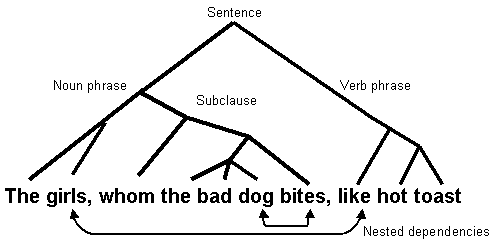
\includegraphics[width=0.6\linewidth]{figure/long-distance-dependency.png}
\label{fig:long-distance-dependency}
\end{figure}

Or:  \\

``The computer which I had just put into the machine room on the fifth
floor crashed.'' 

\end{block}
\end{frame}


%------------------------------------------------
%------------------------------------------------
\begin{frame}\frametitle{N-gram Models}

\begin{block}{Is Markov assumption sufficient? \alert{NO!}}
Language has long-distance dependencies:

\begin{figure}
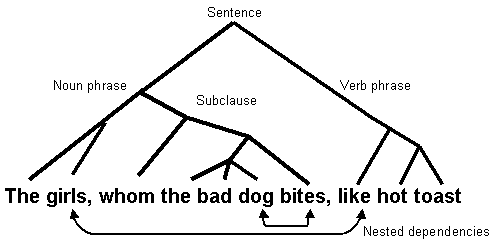
\includegraphics[width=0.6\linewidth]{figure/long-distance-dependency.png}
\label{fig:long-distance-dependency}
\end{figure}

Or:  \\

``The computer which I had just put into the machine room on the fifth
floor crashed.'' 

\end{block}
\end{frame}


%------------------------------------------------
%------------------------------------------------
\begin{frame}\frametitle{N-gram Models}

\begin{block}{Is Markov assumption sufficient? \alert{NO!}}
Language has long-distance dependencies:

\begin{figure}
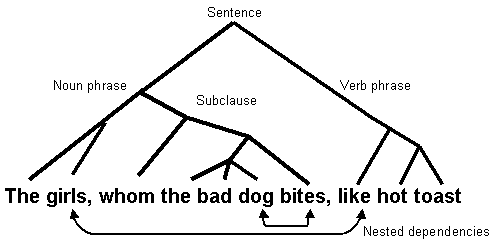
\includegraphics[width=0.6\linewidth]{figure/long-distance-dependency.png}
\label{fig:long-distance-dependency}
\end{figure}

Or:  \\

``The computer which I had just put into the machine room on the fifth
floor crashed.'' 

\end{block}
\end{frame}


%------------------------------------------------
%------------------------------------------------
\begin{frame}\frametitle{N-gram Models}

\begin{block}{Is Markov assumption sufficient? \alert{NO!}}
Language has long-distance dependencies:

\begin{figure}
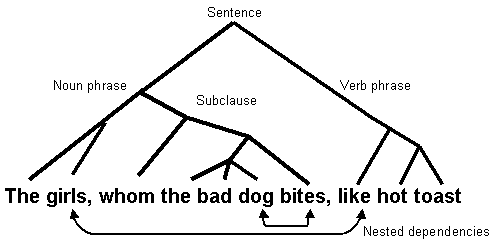
\includegraphics[width=0.6\linewidth]{figure/long-distance-dependency.png}
\label{fig:long-distance-dependency}
\end{figure}

Or:  \\

``The computer which I had just put into the machine room on the fifth
floor crashed.'' 

\end{block}
\end{frame}


%------------------------------------------------
%------------------------------------------------
\begin{frame}\frametitle{N-gram Models}

\begin{block}{Is Markov assumption sufficient? \alert{NO!}}
Language has long-distance dependencies:

\begin{figure}
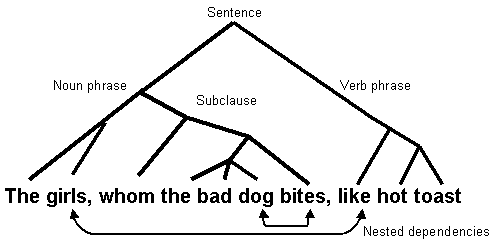
\includegraphics[width=0.6\linewidth]{figure/long-distance-dependency.png}
\label{fig:long-distance-dependency}
\end{figure}

Or:  \\

``The computer which I had just put into the machine room on the fifth
floor crashed.'' 

\end{block}
\end{frame}


%------------------------------------------------
%------------------------------------------------
\begin{frame}\frametitle{N-gram Models}

\begin{block}{Is Markov assumption sufficient? \alert{NO!}}
Language has long-distance dependencies:

\begin{figure}
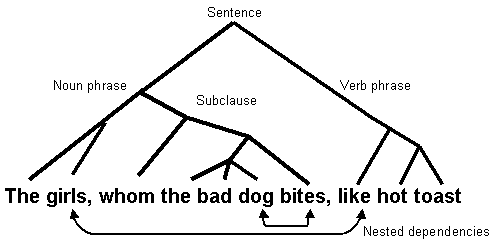
\includegraphics[width=0.6\linewidth]{figure/long-distance-dependency.png}
\label{fig:long-distance-dependency}
\end{figure}

Or:  \\

``The computer which I had just put into the machine room on the fifth
floor crashed.'' 

\end{block}
\end{frame}


%------------------------------------------------
%------------------------------------------------
\begin{frame}\frametitle{N-gram Models}

\begin{block}{Is Markov assumption sufficient? \alert{NO!}}
Language has long-distance dependencies:

\begin{figure}
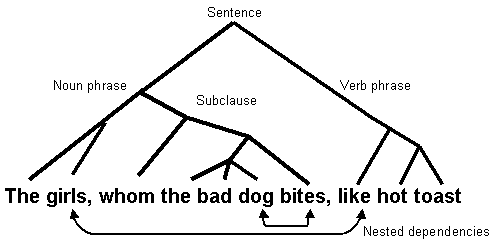
\includegraphics[width=0.6\linewidth]{figure/long-distance-dependency.png}
\label{fig:long-distance-dependency}
\end{figure}

Or:  \\

``The computer which I had just put into the machine room on the fifth
floor crashed.'' 

\end{block}
\end{frame}


%------------------------------------------------
%------------------------------------------------
\begin{frame}\frametitle{N-gram Models}

\begin{block}{Is Markov assumption sufficient? \alert{NO!}}
Language has long-distance dependencies:

\begin{figure}
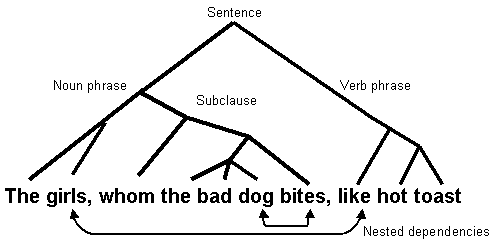
\includegraphics[width=0.6\linewidth]{figure/long-distance-dependency.png}
\label{fig:long-distance-dependency}
\end{figure}

Or:  \\

``The computer which I had just put into the machine room on the fifth
floor crashed.'' 

\end{block}
\end{frame}


%------------------------------------------------
%------------------------------------------------
\begin{frame}\frametitle{N-gram Models}

\begin{block}{Is Markov assumption sufficient? \alert{NO!}}
Language has long-distance dependencies:

\begin{figure}
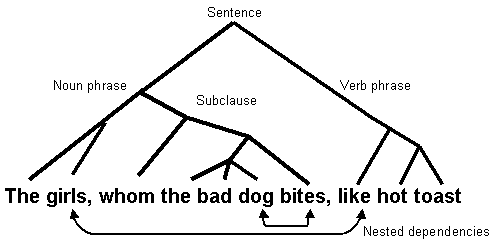
\includegraphics[width=0.6\linewidth]{figure/long-distance-dependency.png}
\label{fig:long-distance-dependency}
\end{figure}

Or:  \\

``The computer which I had just put into the machine room on the fifth
floor crashed.'' 

\end{block}
\end{frame}


%------------------------------------------------
%------------------------------------------------
\begin{frame}\frametitle{N-gram Models}

\begin{block}{Is Markov assumption sufficient? \alert{NO!}}
Language has long-distance dependencies:

\begin{figure}
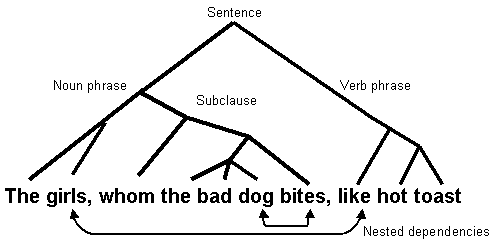
\includegraphics[width=0.6\linewidth]{figure/long-distance-dependency.png}
\label{fig:long-distance-dependency}
\end{figure}

Or:  \\

``The computer which I had just put into the machine room on the fifth
floor crashed.'' 

\end{block}
\end{frame}


%------------------------------------------------







%%%%%%%%%%%%%%%%%%%%%%%%%%%%%%%%%%%%%%%%%%%%%%%%%%%%%%%%%%%%%%%%%%%%%
\section{Size of Language Models}

























% %------------------------------------------------
% \section{First Section} % Sections can be created in order to organize your presentation into discrete blocks, all sections and subsections are automatically printed in the table of contents as an overview of the talk
% %------------------------------------------------

% \subsection{Subsection Example} % A subsection can be created just before a set of slides with a common theme to further break down your presentation into chunks

% \begin{frame}
% \frametitle{Paragraphs of Text}
% Sed iaculis dapibus gravida. Morbi sed tortor erat, nec interdum arcu. Sed id lorem lectus. Quisque viverra augue id sem ornare non aliquam nibh tristique. Aenean in ligula nisl. Nulla sed tellus ipsum. Donec vestibulum ligula non lorem vulputate fermentum accumsan neque mollis.\\~\\

% Sed diam enim, sagittis nec condimentum sit amet, ullamcorper sit amet libero. Aliquam vel dui orci, a porta odio. Nullam id suscipit ipsum. Aenean lobortis commodo sem, ut commodo leo gravida vitae. Pellentesque vehicula ante iaculis arcu pretium rutrum eget sit amet purus. Integer ornare nulla quis neque ultrices lobortis. Vestibulum ultrices tincidunt libero, quis commodo erat ullamcorper id.
% \end{frame}

% %------------------------------------------------

% \begin{frame}
% \frametitle{Bullet Points}
% \begin{itemize}
% \item Lorem ipsum dolor sit amet, consectetur adipiscing elit
% \item Aliquam blandit faucibus nisi, sit amet dapibus enim tempus eu
% \item Nulla commodo, erat quis gravida posuere, elit lacus lobortis est, quis porttitor odio mauris at libero
% \item Nam cursus est eget velit posuere pellentesque
% \item Vestibulum faucibus velit a augue condimentum quis convallis nulla gravida
% \end{itemize}
% \end{frame}

% %------------------------------------------------

% \begin{frame}
% \frametitle{Blocks of Highlighted Text}
% \begin{block}{Block 1}
% Lorem ipsum dolor sit amet, consectetur adipiscing elit. Integer lectus nisl, ultricies in feugiat rutrum, porttitor sit amet augue. Aliquam ut tortor mauris. Sed volutpat ante purus, quis accumsan dolor.
% \end{block}

% \begin{block}{Block 2}
% Pellentesque sed tellus purus. Class aptent taciti sociosqu ad litora torquent per conubia nostra, per inceptos himenaeos. Vestibulum quis magna at risus dictum tempor eu vitae velit.
% \end{block}

% \begin{block}{Block 3}
% Suspendisse tincidunt sagittis gravida. Curabitur condimentum, enim sed venenatis rutrum, ipsum neque consectetur orci, sed blandit justo nisi ac lacus.
% \end{block}
% \end{frame}

% %------------------------------------------------

% \begin{frame}
% \frametitle{Multiple Columns}
% \begin{columns}[c] % The "c" option specifies centered vertical alignment while the "t" option is used for top vertical alignment

% \column{.45\textwidth} % Left column and width
% \textbf{Heading}
% \begin{enumerate}
% \item Statement
% \item Explanation
% \item Example
% \end{enumerate}

% \column{.5\textwidth} % Right column and width
% Lorem ipsum dolor sit amet, consectetur adipiscing elit. Integer lectus nisl, ultricies in feugiat rutrum, porttitor sit amet augue. Aliquam ut tortor mauris. Sed volutpat ante purus, quis accumsan dolor.

% \end{columns}
% \end{frame}

% %------------------------------------------------
% \section{Second Section}
% %------------------------------------------------

% \begin{frame}
% \frametitle{Table}
% \begin{table}
% \begin{tabular}{l l l}
% \toprule
% \textbf{Treatments} & \textbf{Response 1} & \textbf{Response 2}\\
% \midrule
% Treatment 1 & 0.0003262 & 0.562 \\
% Treatment 2 & 0.0015681 & 0.910 \\
% Treatment 3 & 0.0009271 & 0.296 \\
% \bottomrule
% \end{tabular}
% \caption{Table caption}
% \end{table}
% \end{frame}

% %------------------------------------------------

% \begin{frame}
% \frametitle{Theorem}
% \begin{theorem}[Mass--energy equivalence]
% $E = mc^2$
% \end{theorem}
% \end{frame}

% %------------------------------------------------

% \begin{frame}[fragile] % Need to use the fragile option when verbatim is used in the slide
% \frametitle{Verbatim}
% \begin{example}[Theorem Slide Code]
% \begin{verbatim}
% \begin{frame}
% \frametitle{Theorem}
% \begin{theorem}[Mass--energy equivalence]
% $E = mc^2$
% \end{theorem}
% \end{frame}\end{verbatim}
% \end{example}
% \end{frame}

% %------------------------------------------------

% \begin{frame}
% \frametitle{Figure}
% Uncomment the code on this slide to include your own image from the same directory as the template .TeX file.
% %\begin{figure}
% %\includegraphics[width=0.8\linewidth]{test}
% %\end{figure}
% \end{frame}

% %------------------------------------------------

% \begin{frame}[fragile] % Need to use the fragile option when verbatim is used in the slide
% \frametitle{Citation}
% An example of the \verb|\cite| command to cite within the presentation:\\~

% This statement requires citation \cite{p1}.
% \end{frame}

% %------------------------------------------------

% % http://tex.stackexchange.com/questions/147279/references-at-the-end-of-beamer-slides



% \begin{frame}
% \frametitle{References}
% \footnotesize{
% \begin{thebibliography}{99} % Beamer does not support BibTeX so references must be inserted manually as below
% \bibitem[Smith, 2012]{p1} John Smith (2012)
% \newblock Title of the publication
% \newblock \emph{Journal Name} 12(3), 45 -- 678.
% \end{thebibliography}
% }
% \end{frame}

%------------------------------------------------

%------------------------------------------------

% http://tex.stackexchange.com/questions/147279/references-at-the-end-of-beamer-slides



\begin{frame} \frametitle{References}
Many slides are from:
\begin{itemize}
\item StatML book's Web site \&
\item Dan Jurafsky's
``Language Modeling: Introduction to N-grams''. 
\end{itemize}

\end{frame}

%------------------------------------------------
\begin{frame}
\Huge{\centerline{The End}}
\end{frame}

%----------------------------------------------------------------------------------------

\end{document} 